\documentclass[a4paper,12pt]{article}

\usepackage{tabularx} % Для автоподгона ширины
\usepackage{booktabs} % Для красивых линий \toprule, \midrule, \bottomrule
\usepackage[T2A]{fontenc}
\usepackage[utf8]{inputenc}
\usepackage[russian]{babel}
\usepackage{amsmath, amssymb}
\usepackage{graphicx}
\usepackage{geometry}
\usepackage{booktabs}
\geometry{left=30mm,right=15mm,top=20mm,bottom=20mm}
\usepackage{parskip}
\usepackage{amsmath, amssymb}

\title{\textbf{Работа 3. Количественное определение содержания белка в растворе спектрофотометрическим методом}}\\


\begin{document}

\maketitle

\section*{Опыт 1. Спектрофотометрическое определение молярного коэффицента полглощения белка в растворе}

\subsection*{Теоретическая часть}

Определение концентрации белков в растворе методом УФ-спектрометрии основано на поглощении света ароматическими аминокислотными остатками (триптофан, тирозин) и дисульфидными связями в области $280\text{ нм}$.

Молярный коэффициент поглощения белка $\varepsilon_{280}$ при длине волны $280\text{ нм}$ эмпирически расчитывается по формуле:
\[
\varepsilon_{280} = 5500 \cdot n_{\text{Trp}} + 1490 \cdot n_{\text{Tyr}} + 125 \cdot n_{\text{S-S}} \quad [\text{М}^{-1}\text{см}^{-1}],
\]
где $n_{\text{Trp}}$ — число остатков триптофана, $n_{\text{Tyr}}$ — число остатков тирозина, $n_{\text{S-S}}$ — число дисульфидных связей. Вклад дисульфидных связей незначителен и сложно поддается количественной оценке, поэтому слагаемым $(125 \cdot n_{\text{S-S}})$ часто пренебрегают.

В связи с тем, что физическое приготовление $1\text{ М}$ раствора белка невозможно из-за аномально высокой плотности (например, для бычьего сывороточного альбумина (БСА) плотность составила бы $66\text{ кг/л}$), на практике используют величину оптической плотности $0.1\%$-ного раствора ($1\text{ мг/мл}$).

\textbf{Важные примечания:}
\begin{itemize}
    \item При высоких концентрациях белки способны к спонтанной агрегации, что приводит к нарушению закона Бугера--Ламберта--Бера. Пороговая концентрация индивидуальна для каждого белка.
    \item При измерениях в диапазоне $260$--$280\text{ нм}$ необходимо использовать \textbf{кварцевые кюветы}, пропускающие УФ-излучение.
\end{itemize}

\section*{Методика выполнения эксперимента}

\begin{enumerate}
    \item \textbf{Приготовление рабочего раствора:} Путем разбавления исходного раствора большей концентрации дистиллированной водой приготовить $3\text{ мл}$ раствора БСА с концентрацией $1\text{ мг/мл}$ ($0.1\%$).
    \item \textbf{Снятие спектра:} Перенести раствор в кварцевую кювету и записать спектр поглощения в диапазоне длин волн $200$--$400\text{ нм}$.
    \item \textbf{Анализ спектра:} Определить положения максимумов поглощения и зафиксировать значение оптической плотности при длине волны около $280\text{ нм}$ ($A_{280}^{0.1\%}$).
\end{enumerate}

\section*{Обработка результатов и расчет}

\begin{figure}[!htb]
	\centering
	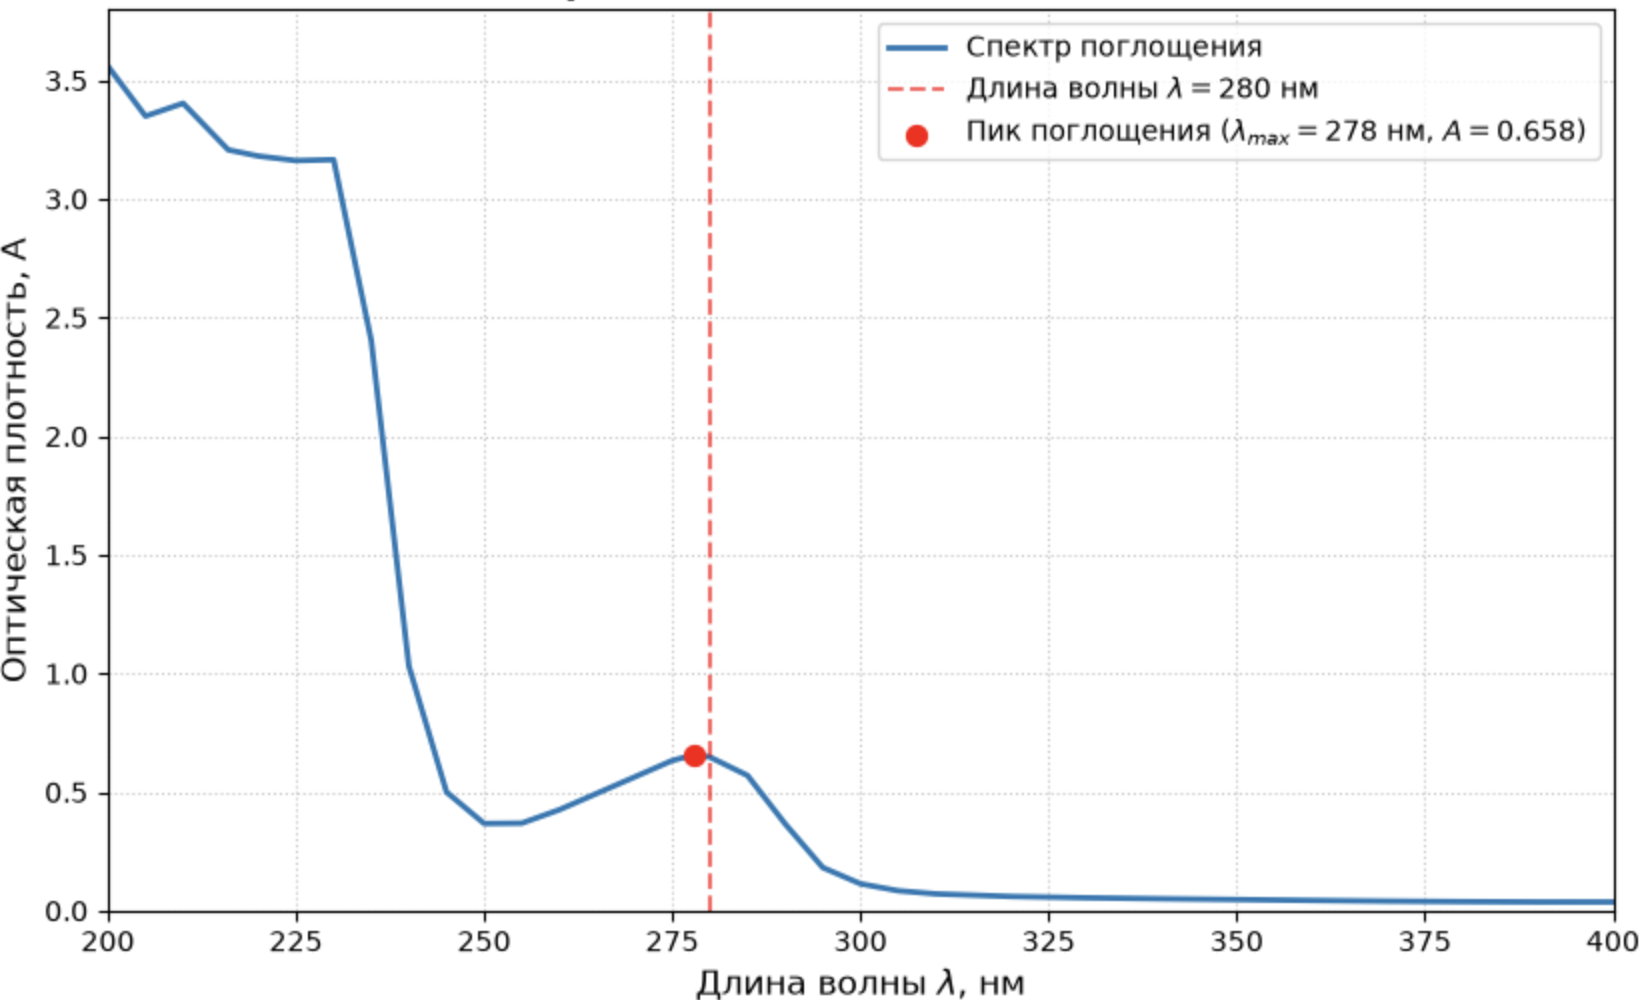
\includegraphics[width=1\textwidth]{BSA.png}
	\caption{Спектр УФ-поглощения BSA}
	\label{fig:sqrt}
\end{figure}

\subsection*{1. Экспериментальные коэффициенты экстинкции при $\lambda = 280$ нм}

По исходным данным из измерений при $\lambda = 280\text{ нм}$:
\begin{itemize}
    \item Оптическая плотность при концентрации $c_m = 1\text{ мг/мл}$: $A_{280} = 0.6473$.
    \item Длина оптического пути: $l = 1\text{ см}$.
    \item Молярная масса BSA: $M = 66.4\text{ кДа} = 66\,400\text{ г/моль}$.
\end{itemize}

\textbf{Массовый коэффициент экстинкции ($E^{1\%}_{1\,\text{cm}}$ и $\varepsilon_{m}$):}

Массовый коэффициент экстинкции $\varepsilon_{m}$ для концентрации $1\text{ мг/мл}$ ($0.1\%$ раствор):
\[
\varepsilon_{m} = \frac{A_{280}}{c_m \cdot l} = \frac{0.6473}{1\text{ мг/мл} \cdot 1\text{ см}} = 0.6473\text{ мл}\cdot\text{мг}^{-1}\cdot\text{см}^{-1} = 0.6473\text{ л}\cdot\text{г}^{-1}\cdot\text{см}^{-1}
\]

Значение $E^{1\%}_{1\,\text{cm}}$ (для $10\text{ мг/мл}$ раствора):
\[
E^{1\%}_{1\,\text{cm}} = \varepsilon_{m} \times 10 = 6.473\text{ \%}^{-1}\cdot\text{см}^{-1}
\]

\newpage
\textbf{Экспериментальный молярный коэффициент экстинкции ($\varepsilon_{\text{практ}}$):}

Переведем массовую концентрацию $1\text{ мг/мл} = 1\text{ г/л}$ в молярную $C_{\text{моль}}$:
\[
C_{\text{моль}} = \frac{c_m}{M} = \frac{1\text{ г/л}}{66\,400\text{ г/моль}} \approx 1.50602 \times 10^{-5}\text{ моль/л}
\]

Используя закон Бугера — Ламберта — Бера ($A = \varepsilon \cdot C \cdot l$):
\[
\varepsilon_{\text{практ}} = \frac{A_{280}}{C_{\text{моль}} \cdot l} = \frac{0.6473}{1.50602 \times 10^{-5}\text{ моль/л} \cdot 1\text{ см}} \approx 42\,981\text{ М}^{-1}\cdot\text{см}^{-1}
\]

\subsection*{2. Теоретический расчет молярного коэффициента экстинкции ($\varepsilon_{\text{теор}}$)}

Теоретический молярный коэффициент экстинкции денатурированного/непосредственно рассчитанного белка при $\lambda = 280\text{ нм}$ вычисляется по формуле Пасе и Прэтта (Pace et al.):
\[
\varepsilon_{\text{теор}} = n_{\text{Trp}} \cdot \varepsilon_{\text{Trp}} + n_{\text{Tyr}} \cdot \varepsilon_{\text{Tyr}} + n_{\text{cystine}} \cdot \varepsilon_{\text{cystine}}
\]

Где стандартные значения молярных коэффициентов при $280\text{ нм}$:
\begin{itemize}
    \item $\varepsilon_{\text{Trp}} = 5500\text{ М}^{-1}\cdot\text{см}^{-1}$
    \item $\varepsilon_{\text{Tyr}} = 1490\text{ М}^{-1}\cdot\text{см}^{-1}$
    \item $\varepsilon_{\text{cystine}} = 125\text{ М}^{-1}\cdot\text{см}^{-1}$ (для дисульфидных связей $\text{S–S}$)
\end{itemize}

В структуре БСА присутствуют 17 остатков цистеина, образованные в дисульфидные мостики. Количество дисульфидных связей $n_{\text{cystine}} = \frac{17}{2} = 8.5$:

\[
\varepsilon_{\text{теор}} = 2 \cdot 5500 + 20 \cdot 1490 + 8.5 \cdot 125
\]
\[
\varepsilon_{\text{теор}} = 11\,000 + 29\,800 + 1062.5 = 41\,862.5\text{ М}^{-1}\cdot\text{см}^{-1}
\]

\subsection*{3. Оценка оптической плотности для концентрации $10\text{ мг/мл}$}

При концентрации $c_m = 10\text{ мг/мл}$ молярная концентрация белка составляет:
\[
C_{\text{моль}} = \frac{10\text{ г/л}}{66\,400\text{ г/моль}} \approx 1.50602 \times 10^{-4}\text{ М}
\]

\textbf{1) Практическое значение оптической плотности ($A_{\text{практ}}$):}
\[
A_{\text{практ}} = \varepsilon_{\text{практ}} \cdot C_{\text{моль}} \cdot l = 42\,981 \cdot 1.50602 \times 10^{-4} \cdot 1 = 6.473
\]

\textbf{2) Теоретическое значение оптической плотности ($A_{\text{теор}}$):}
\[
A_{\text{теор}} = \varepsilon_{\text{теор}} \cdot C_{\text{моль}} \cdot l = 41\,862.5 \cdot 1.50602 \times 10^{-4} \cdot 1 \approx 6.305
\]

\newpage 


\section*{Опыт 2. Колориметрическое определение концентрации белка при
помощи биуретового реактива}

\section*{Теоретическая часть}

\textbf{Биуретовая реакция} — классический фотометрический метод количественного определения белка.

\textbf{Принцип метода:} В щелочной среде ионы меди $\text{Cu}^{2+}$, входящие в состав биуретового реактива, образуют с пептидными связями ($-\text{CO}-\text{NH}-$) белков и пептидов устойчивый координационный комплекс красновато-фиолетового цвета с максимумом поглощения при $\lambda \approx 545\text{ нм}$.


\subsection*{Методика выполнения работы}

\begin{enumerate}
    \item Путем разбавления дистиллированной водой исходного раствора БСА приготовили в микропробирках по $1\text{~мл}$ стандартных растворов с концентрациями $1$, $3$, $5$, $7$ и $9\text{~мг/мл}$.
    \item Получили у преподавателя контрольный раствор БСА (AMX) с неизвестной концентрацией.
    \item В отдельные микропробирки внесли реагенты согласно Таблице~1 (для «холостой» пробы $1000\text{ мкл}$ воды и $200\text{ мкл}$ биуретового реактива; для калибровочных и контрольной проб — $800\text{ мкл}$ воды, $200\text{ мкл}$ соответствующего раствора белка и $200\text{ мкл}$ биуретового реактива).
    \item Инкубировали пробы при комнатной температуре в течение $15\text{ минут}$ до полного развития красно-фиолетовой окраски.
    \item Измерили оптическую плотность $A$ при $\lambda = 545\text{ нм}$ относительно «холостой» пробы.
\end{enumerate}

\section*{Обработка результатов и расчет}

Максимум оптической плотности неизвестного образца: $A_{\max} = 0.0273$.

\begin{enumerate}
    \item \textbf{Калибровка по линейному диапазону ($1\text{--}5\text{ мг/мл}$):}
    Уравнение прямой:
    \begin{equation*}
        A = 0.0238 \cdot C - 0.0756 \quad (R^2 = 0.922)
    \end{equation*}
    Расчет концентрации:
    \begin{equation*}
        C = \frac{0.0273 + 0.0756}{0.0238} \approx \mathbf{4.33\text{ мг/мл}}
    \end{equation*}

    \item \textbf{Калибровка по всем 5 точкам ($1\text{--}9\text{ мг/мл}$):}
    Уравнение прямой:
    \begin{equation*}
        A = 0.0113 \cdot C - 0.0432 \quad (R^2 = 0.708)
    \end{equation*}
    Расчет концентрации:
    \begin{equation*}
        C = \frac{0.0273 + 0.0432}{0.0113} \approx \mathbf{6.25\text{ мг/мл}}
    \end{equation*}
\end{enumerate}

\begin{table}[h!]
\centering
\caption{Схема приготовления реакционных смесей для биуретовой реакции}
\label{tab:biuret_prep}
\vspace{0.2cm}
\begin{tabular}{l c c c c}
\toprule
\textbf{Проба} & \textbf{\begin{tabular}[c]{@{}c@{}}Концентрация БСА,\\ мг/мл\end{tabular}} & \textbf{\begin{tabular}[c]{@{}c@{}}$V(\text{H}_2\text{O})$,\\ мкл\end{tabular}} & \textbf{\begin{tabular}[c]{@{}c@{}}$V(\text{раствора белка})$,\\ мкл\end{tabular}} & \textbf{\begin{tabular}[c]{@{}c@{}}$V(\text{реактива})$,\\ мкл\end{tabular}} \\
\midrule
Контроль «0» & 0 & 1000 & — & 200 \\
Стандарт 1 & 1 & 800 & 200 & 200 \\
Стандарт 2 & 3 & 800 & 200 & 200 \\
Стандарт 3 & 5 & 800 & 200 & 200 \\
Стандарт 4 & 7 & 800 & 200 & 200 \\
Стандарт 5 & 9 & 800 & 200 & 200 \\
Проба AMX & $C_x$ & 800 & 200 & 200 \\
\bottomrule
\end{tabular}
\end{table}

\end{document}
